Expressions describing or referring to objects in visual scenes typically include a word naming the type of the object: e.g.,  \emph{cheesecake} or  \emph{dessert}  in Figure~\ref{fig:ex1}. 
Determining these objects names is a core aspect of virtually every language \& vision task, ranging from e.g.\ referring expression generation to visual dialogue.
Nevertheless, research in language \& vision has mostly  sidestepped questions about how speakers actually choose these names and how computational models should account for it.



While state-of-the-art computer vision systems are able to accurately classify images into thousands of different categories (e.g.\  \newcite{googlenet}), they mostly adopt very simple assumptions with respect to the underlying lexicon, which is typically implemented as a simple, flat labeling scheme. Thus, a standard object recognition system would be trained to classify the objects in Figure~\ref{fig:cake} as either  \emph{dessert} or \emph{cake}.
In contrast, humans seem to be more flexible as to the chosen level of generality and to the chosen part of the taxonomy (see objects in Figure \ref{fig:cake} that could be named \refexp{cake}, \refexp{cheesecake}, \refexp{dessert}, \refexp{sweet}, \refexp{pastry}, \refexp{food} etc.) 
Seminal work on prototypes suggests that the prototypicality of the object will determine the level of generality of the object name, i.e.\  a robin can be named \emph{bird}, but a penguin is better referred to as ``\emph{penguin}'' \cite{Rosch1978}.

%To date, surprisingly little work has been done on testing such theoretical predictions on large-scale, language \& vision data sets and integrating them explicitly into modeling frameworks.

\begin{figure}[htbp]
\begin{center}
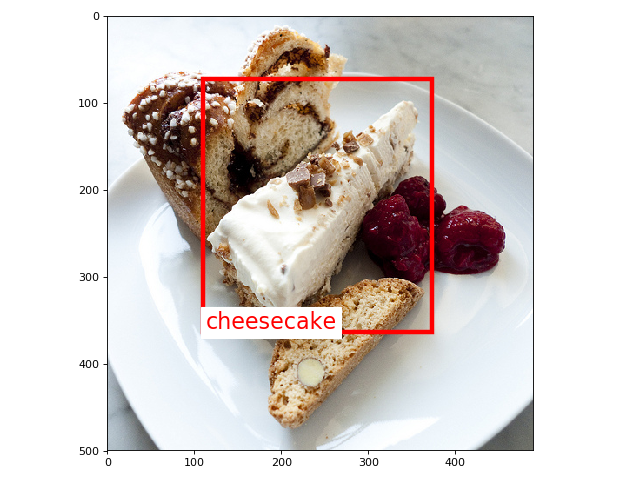
\includegraphics[height=3cm]{figures/cheesecake.png}
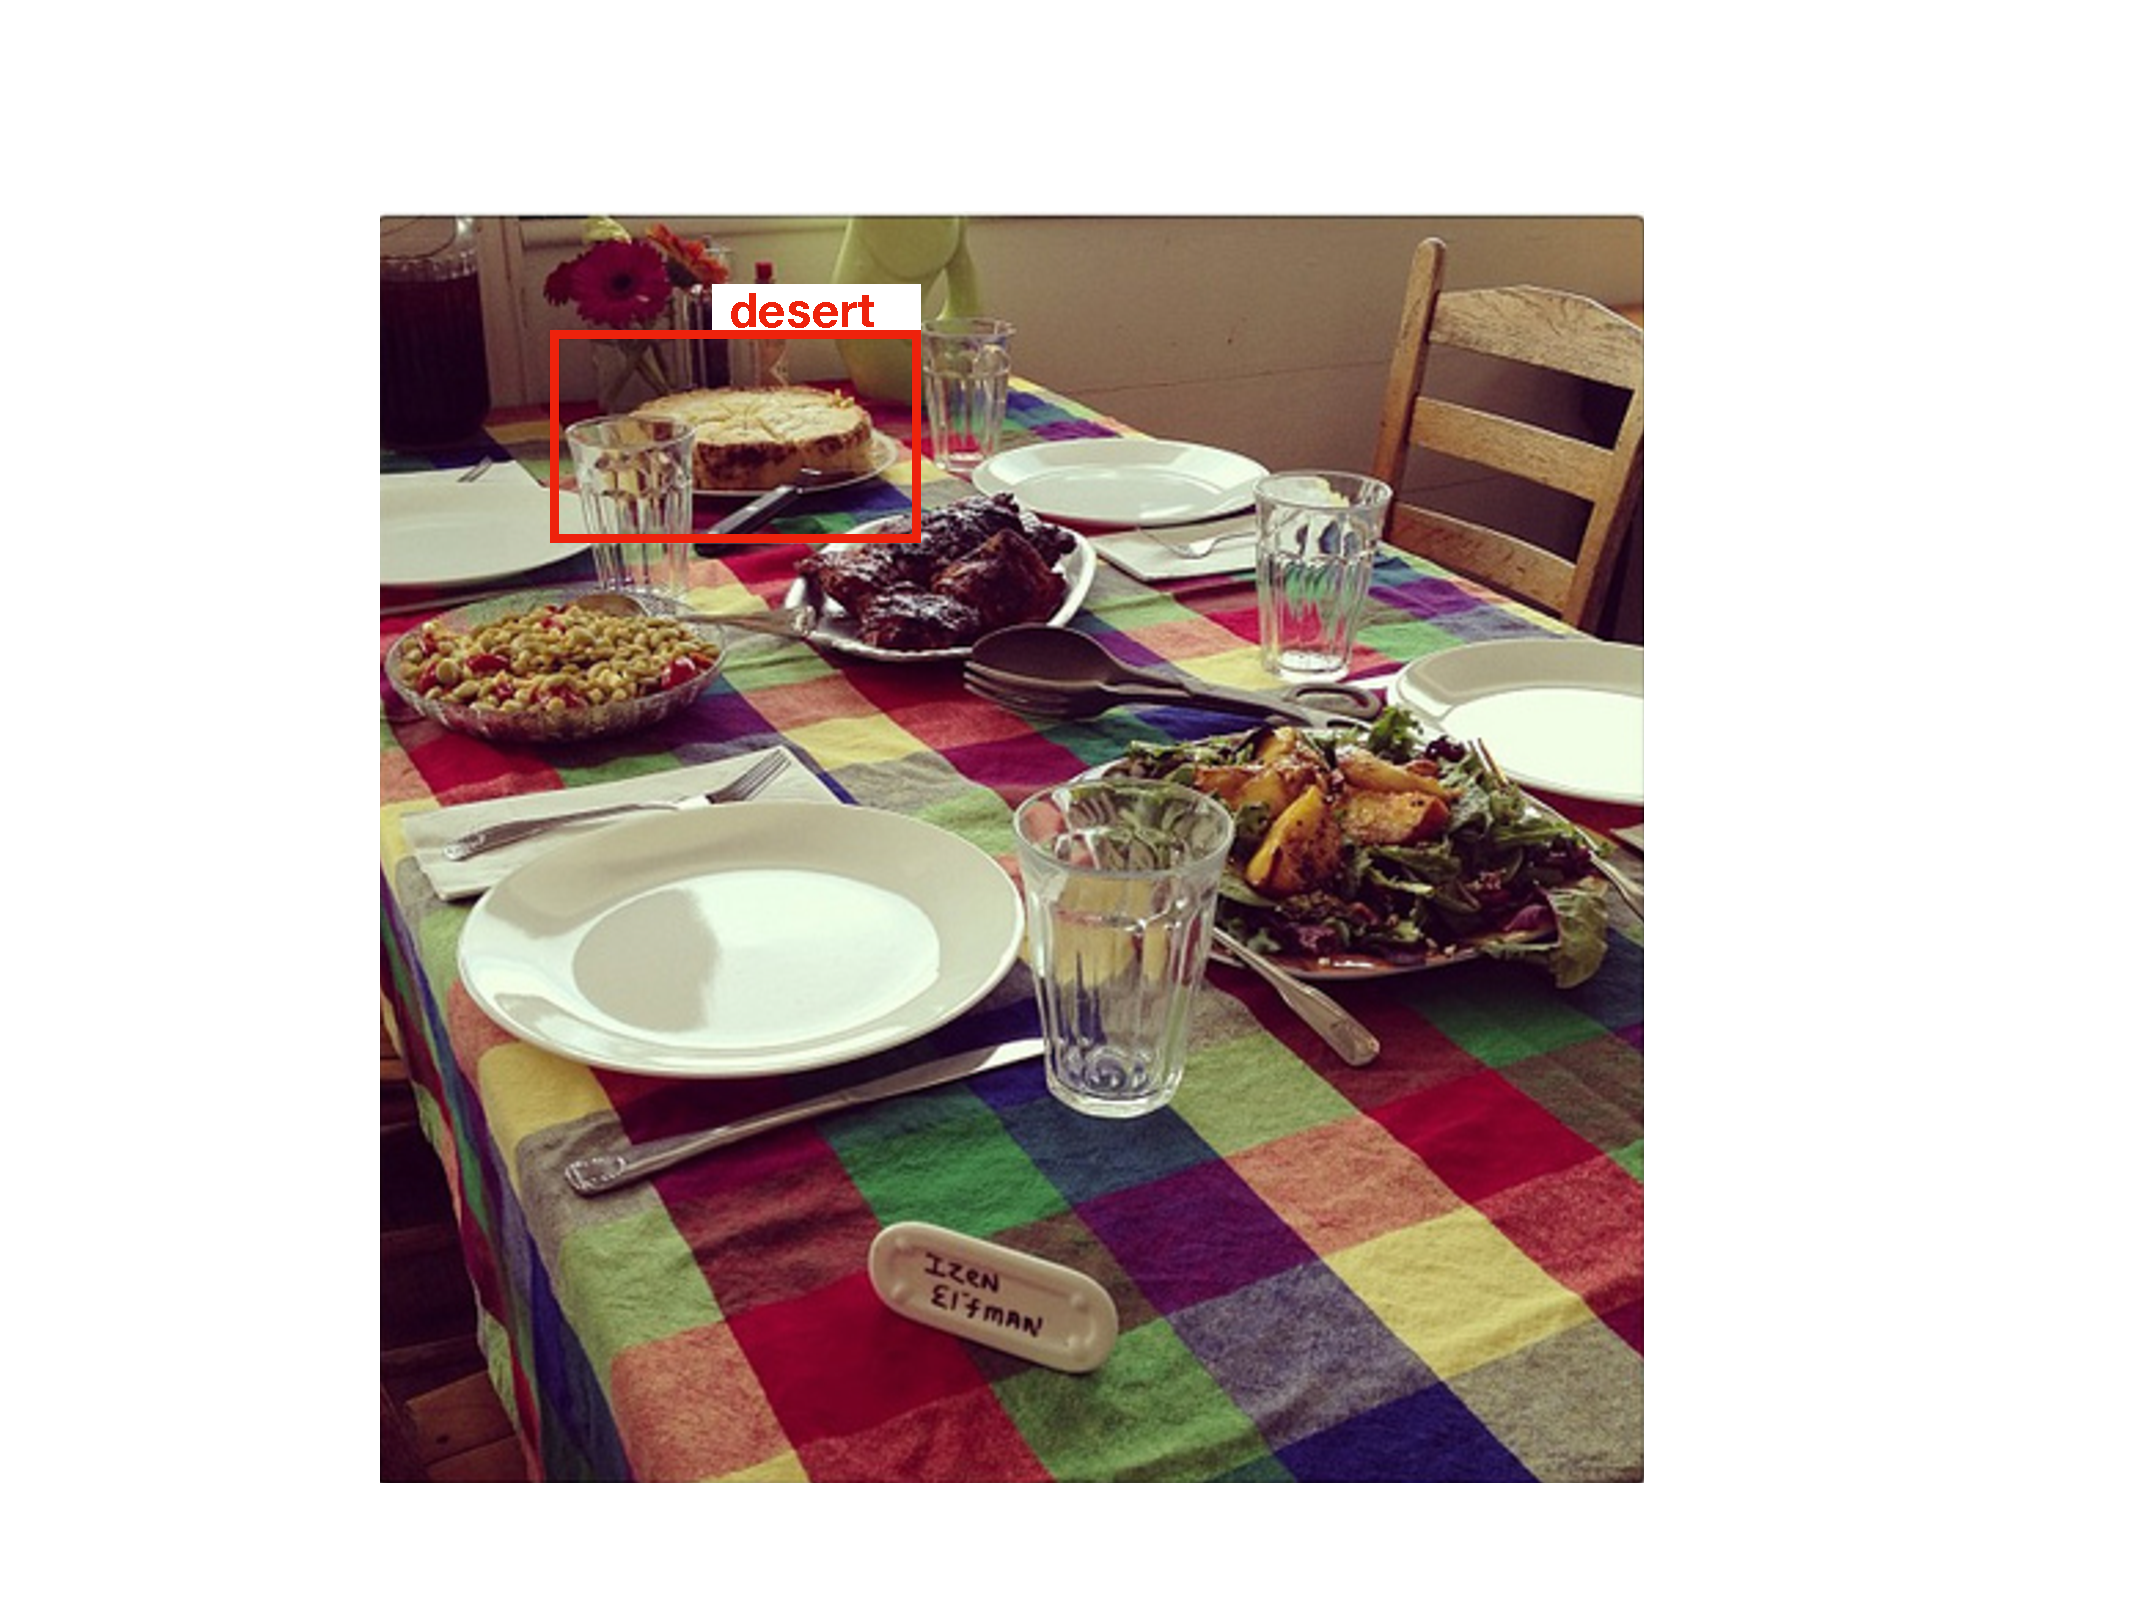
\includegraphics[height=3cm]{figures/cheesecak2.pdf}
\caption{Two objects of the same type of cake, with different names in VisualGenome}
\label{fig:cake}
\end{center}
\end{figure}

Two main findings in the literature:

\begin{itemize}
\item very high agreement, most people use the same name for the same object
\item prototypicality is a factor, context too, but research has only looked at generality/specificity of the name
\end{itemize}


\sz{something is missing here .. explain why exactly we did what we did, why is it interesting to collect many names for the same object?}

There are two main findings:

\begin{itemize}
\item the level of agreement in object naming is much higher in certain domains than in others, as it happens, the domains that have been traditionally used in object naming research (e.g. animals) seem to display the highest amount of agreement in our data set 
\item while previous work has mostly focussed on variation in the level of generality (\emph{penguin} vs. \emph{bird}), our datasets contains a lot of variability for names coming from different parts of the taxonomy (\emph{dessert} vs. \emph{cake}, \emph{bottle} vs. \emph{wine})
\end{itemize}


%The real-world objects that we interact with in our every-day life can be categorized into many thousands and maybe millions of categories. And even a single object can be member of many categories, i.e.\ at different taxonomical levels or in different parts of a taxonomy. For instance, both objects in Figure \ref{fig:cake} are at once instances of \cat{cake}, \cat{cheesecake}, \cat{dessert}, \cat{sweet}, \cat{pastry}, \cat{food} etc. Hence, when speakers name objects, e.g.\ when referring, they have to select a lexical item from a complex network of concepts and competing lexical alternatives.




%To date, research in NLP has surprisingly little to say about object naming, despite the fact that
% there has been a recent explosion of interest in various, and even complex, language \& vision tasks ranging from image captioning \cite{fangetal:2015,devlin:imcaqui,Bernardietal:automatic} to e.g.\ visual dialogue \cite{das2017visual,vries2017guesswhat}. 
%In contrast, closely related areas, such as computer vision and cognitive science, have investigated very related tasks in quite some depth: object recognition systems developed in the area of computer vision  are now able to classify images into thousands of different categories (e.g.\  \newcite{googlenet}).
%Furthermore, work on concepts, following the seminal work by Rosch, suggests that objects are typically conceptualized at a preferred level of specificity called the \textbf{entry-level}. Psycho-linguistic studies have been able to support this theory based on collections of so-called object naming norms. 
%
%This paper aims at addressing the genuinely linguistic questions revolving around the phenomenon of object naming by (i) presenting a collection of high-quality, large-scale naming data,  and (ii) analysis methods for this data and (iii) a first baseline model that accounts for the semantic flexibility of names for objects in real-world images. From computer vision, we borrow the idea of modeling realistic visual objects in realistic scenes (real-world images), but go beyond the simplistic assumption that object names correspond to unambiguous labels in a flat classification scheme (with no conceptual relations between the labels). From psycholinguistics, we borrow the idea of eliciting natural, representative naming data from many subjects, but go beyond using artificial, highly stylized objects.

%%% Local Variables:
%%% mode: latex
%%% TeX-master: "main"
%%% End:
